\section{Elektromagnet}
Elektromagneten er lavet til at holde bilen på banen. Ved at aktivere elektromagneten i sving, burde den optimere bilens evne til at holde sig på banen ved højere hastighed end uden elektromagnet.

\subsection{Kernemateriale}
En vigtig faktor i fremstilling af elektromagneter er materialet. Ud fra materialet bestemmes elektromagnetens magnetiske evne. Materialets permeabilitet bestemmer hvor godt det kan lede et magnetisk felt. Permeabiliteten kan deles op i tre underemner, ferromagnetisk, paramagnetisk og diamagnetisk. Det kan ses i figur \ref{Permeabilitet}. \\
\begin{wrapfigure}{r}{0.5\textwidth}
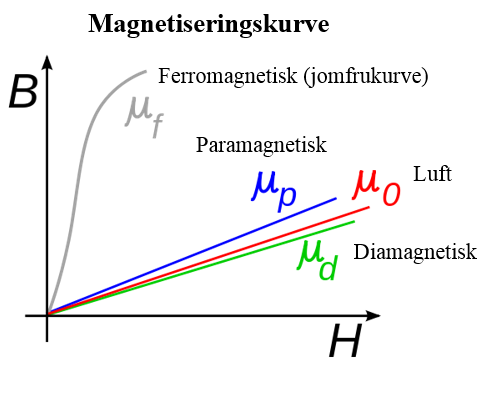
\includegraphics[scale=0.4]{./Graphics/Magnetiseringskurve}
\caption{Permeabilitete i forskellige materialer}
\label{Permeabilitet}
\end{wrapfigure}
I diamagnetiske materialer er magnetiseringen ekstremt lille og har en lineær HB-kurve. Ved paramagnetiske materialer er magnetiseringen ligeledes meget lille, men større end diamagnetiske materialer og ligeledes har materialet en lineær HB-kurve\footnote{Se ordlist i afsnit \ref{ordliste}}. Ferromagnetiske materialer har en stor magnetisering, den magnetiske effekt skyldes herved de uparrede elektroner der forekommer i nogle metaller. Ferromagnetiske materialer har en logistisk stigende HB-kurve.\\

Ferromagnetisk materiale kan nu deles op i to undergrupper, blødt materiale og hårdt materiale. Blødt materiale er karakteriseret ved høj permeabilitet, lille hysteresekurve med et lille koercivt felt og lavt kulstofindhold. Bløde materialer er ofte en legering af jern og silicium eller nikkel. \\
\begin{wrapfigure}{r}{0.5\textwidth}
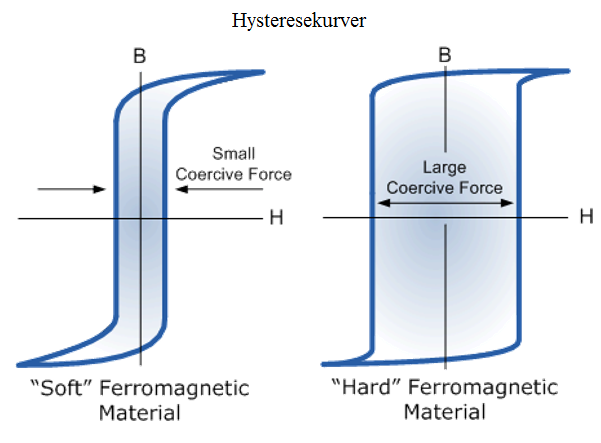
\includegraphics[scale=0.4]{./Graphics/Hysteresekurver}
\caption{Hysteresekurve på blødt og hårdt ferromagnetisk materiale}
\label{Hysteresekurve}
\vspace{-110pt}
\end{wrapfigure}
Hårdt materiale er karakteriseret ved mindre permeabilitet end blødt materiale, bred hysteresekurve, stort koercivt felt og højt kulstofindhold. Hårde materialer er ofte en legering af jern med kulstof, aluminium eller wolfram. Se figur \ref{Hysteresekurve}. 

\newpage
\subsection{Prøvemagnet}
Som udgangspunkt er kernematerialet blevet antaget til at være stål, da materialet er ferromagnetisk og hårdt. Hvis der skulle laves en korrekt undersøgelse at kernematerialet ville det kræve en længere og meget tidskrævende undersøgelse, derfor har dette kun været en overvejelse. \\
Næste overvejelse har været placering og form af elektromagneten. Der er tre steder elektromagneten kan placeres på bilen; foran, bagpå eller under bilen.\\
\begin{figure}[h!]
\center
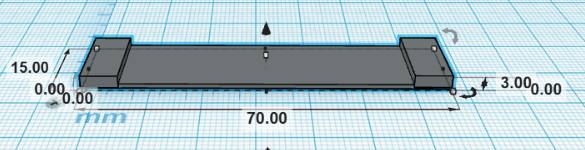
\includegraphics[scale=0.4]{./Graphics/Elektromagnet_2D}
\caption{Skabelon over elektromagneten med aktuelle mål}
\label{Elektromagnet_skabelon}
\end{figure}

Hverken trække eller skubbe elektromagneten er en effektiv løsning, det vil skabe uligevægt i bilen og flytte massemidtpunktet. Ved en stærk elektromagnet vil man ændre friktionskraften meget ved at montere elektromagneten foran eller bagved. Hvis elektromagneten sidder bagpå vil der opstå meget friktion på baghjulene og mindre friktion på forhjulene.\\
Fluxspredning (Se figur \ref{Flux}) er en faktor der skal tages hensyn til når formen af elektromagneten laves. Der vil altid være fluxspredning men formen kan være med til at reducere det betydeligt. Fluxlinjerne bevæger sig fra nord til syd. For fuld udnyttelse af elektromagneten bør nord- og sydpol befinde sig over skinnerne således at fluxlinjerne løber langs skinnerne. Hvis elektromagneten formes som en hestesko vil nord og syd pege ned mod skinnerne. For at undgå for meget fluxspredning bør fordybningen i hesteskoen være så stor som mulig. Se journalen i bilag \ref{Elektrojournal}.\\

\begin{wrapfigure}{r}{0.5\textwidth}
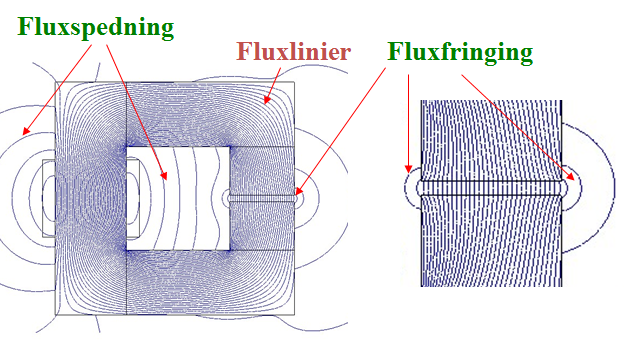
\includegraphics[scale=0.4]{./Graphics/Flux}
\caption{Flux, fluxfringing, fluxspredning}
\label{Flux}
\end{wrapfigure}

Efter valg af materiale, placering og form, skal antal vindinger bestemmes. Grunden afstanden mellem bilens undervogn og vejen, vil der kun være plads til cirka 660 vindinger. Hvis elektromagneten er tykkere er der, pga. affjedringen, risiko for at kortslutte banen.\\
\\
Testmagneten er lavet ud fra de forrige overvejelser og formlen for den magnetiske kraft i et luftgab (under idelle forhold). Denne kraft er givet ved:\\
\\
$F_{magn}(x)=-{\frac{B^{2}_{g}}{2\mu_{0}}}* {A_{j}}* (\frac{4x}{{\frac{l_{j}}{\mu_{r}}}+2x}-1) $
%$ {{\frac{4x}}{{frac{\l_{j}}{\mu_{r}}}}+2x}-1 $
\\
\\
Hvor $B_{g}$ er:
\\
\\
$ B_{g}(x)=\frac{\mu_{0}IN}{{\frac{l_{j}}{\mu_{r}}}+2x} $
\\
\\
Ud fra de overstående ligninger er magnetkraften fundet til at være 1,309N. I praksis er den målt, med et newtonmeter, til at være cirka 0,9367N. Se evt. nærmere i bilag \ref{Elektrojournal}. \\
Da 0,9367N er en meget lille kraft, bør det overvejes grundigt om elektromagneten vil være en ulempe eller fordel for bilen. Det er blevet beregnet hvor hurtigt man kan køre med og uden elektromagneten i svingene. Dette kan der læses mere om i afsnit \ref{sving}.\\
